\chapter{Detailed RAG Implementation}

This appendix collects the lower-level implementation details, intermediate data representations, and supporting screenshots for the RAG subsystem described at a higher level in Chapter 4. It is intended as supporting engineering documentation rather than the main narrative of the final report.

\section{Implemented Retrieval Server Interfaces}
Table \ref{tab:retrieval-server-interfaces} provides a compact summary of the main retrieval server interfaces implemented for integration with Meadow9+. The table is intended to demonstrate implementation coverage at a high level without reproducing the full API contract in the body chapters.

\begin{table}[H]
  \centering
  \setlength{\tabcolsep}{5pt}
  \renewcommand{\arraystretch}{1.15}
  \begin{tabular}{|l|l|>{\raggedright\arraybackslash}p{0.36\textwidth}|}
    \hline
    \textbf{Method} & \textbf{Interface Category} & \textbf{Purpose} \\
    \hline
    GET & Service metadata & Expose basic service metadata, documentation entry points, and service discovery information for integration. \\
    \hline
    GET & Health monitoring & Report runtime readiness, retrieval initialization state, and dependency availability so failures can be detected operationally. \\
    \hline
    POST & Transcript ingestion & Accept uploaded transcript input for validation, parsing, chunking, summarization, persistence, and indexing into the retrieval layer. \\
    \hline
    GET & Transcript listing and retrieval & List available transcripts and return stored transcript summaries or raw transcript content for application use. \\
    \hline
    POST & Keyword-based search & Execute corpus-level transcript search and return grouped transcript-level matches with supporting chunks. \\
    \hline
    POST & One-off query & Perform stateless grounded question answering over the uploaded transcript corpus. \\
    \hline
    POST & Multi-turn chat & Support transcript-aware conversational question answering with retrieved evidence returned alongside the generated answer. \\
    \hline
    POST & Streaming chat & Stream partial chat responses to reduce perceived latency while returning final retrieval metadata at completion. \\
    \hline
    GET / DELETE & Session management & List active chat sessions or delete a session when conversation state should be cleared. \\
    \hline
  \end{tabular}
  \caption{High-level summary of implemented retrieval server interfaces}
  \label{tab:retrieval-server-interfaces}
\end{table}

\section{Transcript Parsing, Chunking, and Storage}
The RAG ingestion path begins by parsing SRT transcripts into structured records containing text, timestamps, sequence numbers, and speaker metadata. Speaker detection handles both simple markers and explicit speaker-name prefixes so that speaker information can later be used for filtering and citation without polluting the searchable transcript text.

\begin{figure}[H]
  \centering
  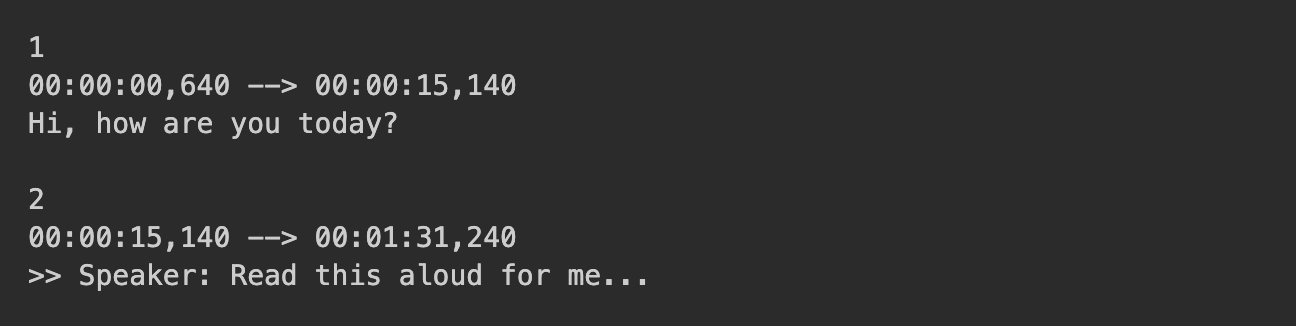
\includegraphics[width=1.0\textwidth]{figures/srt_input_format_with_sequence_numbers_and_timestamps.png}
  \caption{SRT input format with sequence numbers and timestamps}
  \label{fig:fig18}
\end{figure}

\begin{figure}[H]
  \centering
  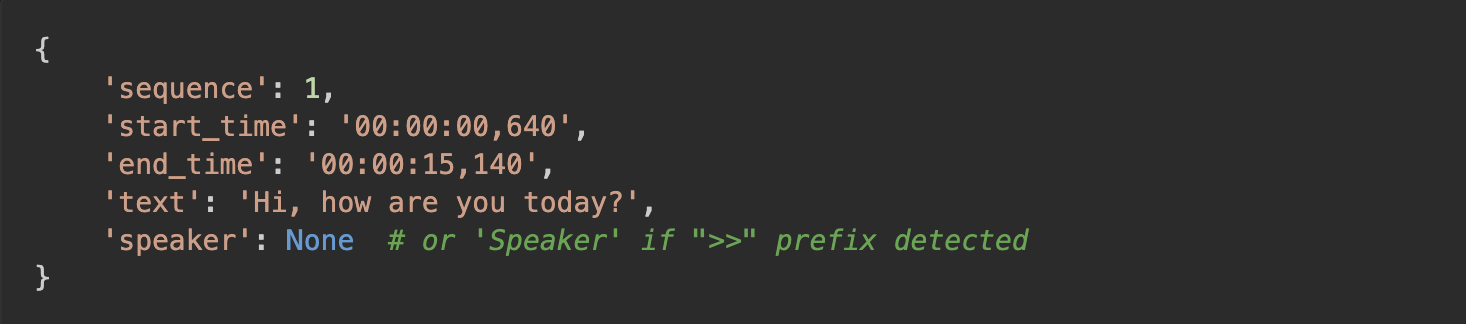
\includegraphics[width=1.0\textwidth]{figures/parsed_srt_structure_with_speaker_metadata_extraction.png}
  \caption{Parsed SRT structure with speaker metadata extraction}
  \label{fig:fig19}
\end{figure}

After parsing, small subtitle units are merged into retrieval-sized chunks using token-counted boundaries. This is more reliable than character-based estimation because it aligns chunk sizing with the practical limits of the embedding and generation models, while preserving natural subtitle boundaries for later timestamp attribution and answer grounding.

\begin{figure}[H]
  \centering
  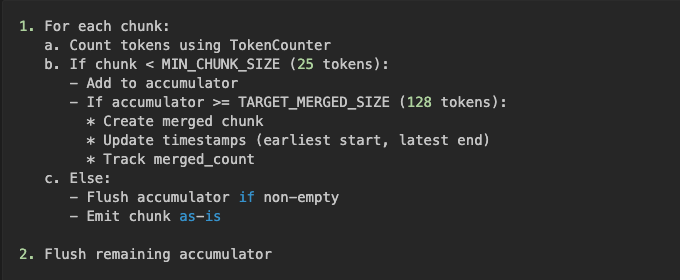
\includegraphics[width=1.0\textwidth]{figures/token_based_merging_algorithm_for_chunk_size_optimization.png}
  \caption{Token-based merging algorithm for chunk size optimization}
  \label{fig:fig20}
\end{figure}

The merged chunks are then converted into LangChain `Document` objects with transcript identifiers, timestamps, chunk IDs, and speaker information attached as metadata. This representation is used consistently across retrieval, reranking, filtering, and citation formatting.

\begin{figure}[H]
  \centering
  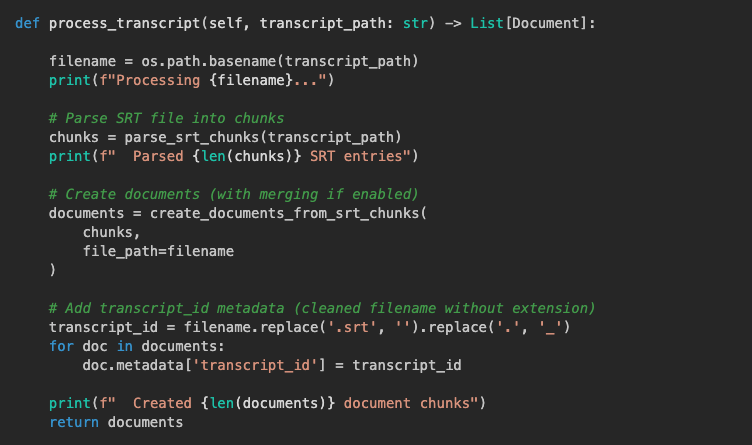
\includegraphics[width=1.0\textwidth]{figures/document_processing_pipeline.png}
  \caption{Document processing pipeline}
  \label{fig:fig24f}
\end{figure}

Embedding generation is one of the most computationally expensive stages in indexing, so the implementation relies on batched vector-store integration rather than one document at a time. Chroma persists the resulting embeddings and metadata in local storage, while incremental addition supports appending newly uploaded transcripts without rebuilding the entire index.\cite{langchain_chroma,chroma_persistence_sqlite}

\begin{figure}[H]
  \centering
  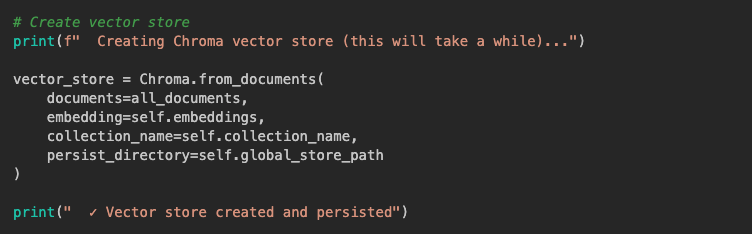
\includegraphics[width=1.0\textwidth]{figures/vector_store_creation_from_documents.png}
  \caption{Vector store creation from documents}
  \label{fig:fig25d}
\end{figure}

\begin{figure}[H]
  \centering
  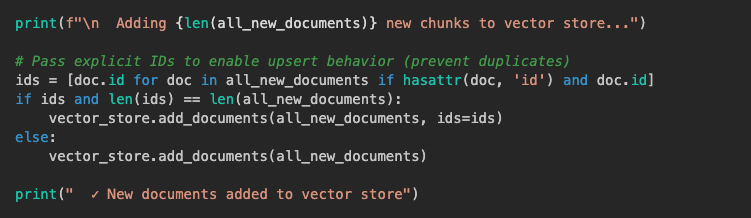
\includegraphics[width=1.0\textwidth]{figures/incremental_document_addition.png}
  \caption{Incremental document addition}
  \label{fig:fig25e}
\end{figure}

\begin{figure}[H]
  \centering
  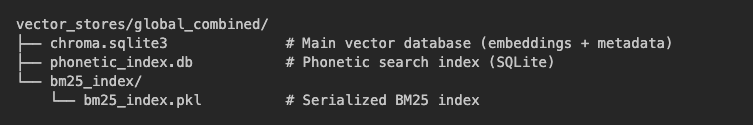
\includegraphics[width=1.0\textwidth]{figures/chromadb_storage_directory_structure.png}
  \caption{ChromaDB storage directory structure}
  \label{fig:fig26a}
\end{figure}

\section{Hybrid Retrieval Internals and Reranking}
Stage 1 retrieval combines four complementary signals: dense vector search for semantic similarity, BM25 for exact lexical evidence, phonetic search for ASR-induced spelling distortions, and fuzzy matching for character-level corruption in rare tokens.\cite{robertson2009bm25,black2021doublemetaphone,levenshtein1965,jina_embeddings_v3}

Vector search operates over dense embeddings stored in Chroma and supports optional metadata filtering for transcript-scoped retrieval.

\begin{figure}[H]
  \centering
  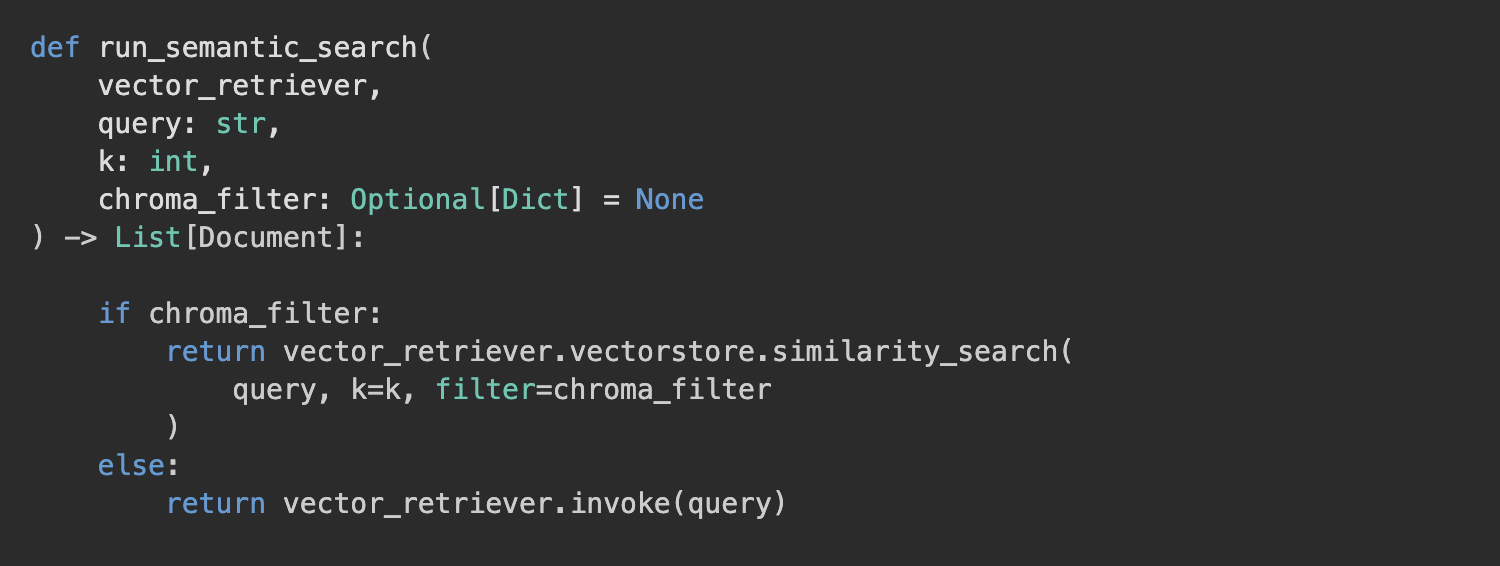
\includegraphics[width=1.0\textwidth]{figures/vector_search_core_function_showing_semantic_retrieval_with_optional_c.png}
  \caption{Vector search core function showing semantic retrieval with optional metadata filtering}
  \label{fig:fig27a}
\end{figure}

BM25 provides exact keyword matching and is especially useful for proper nouns, brands, acronyms, and technical terms that should appear verbatim in the retrieved evidence.

\begin{figure}[H]
  \centering
  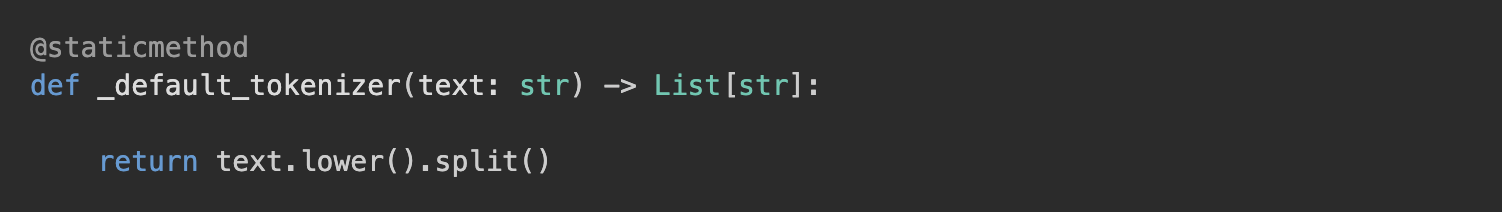
\includegraphics[width=1.0\textwidth]{figures/bm25_tokenization_function_using_lowercase_split.png}
  \caption{BM25 tokenization function using lowercase split}
  \label{fig:fig28a}
\end{figure}

\begin{figure}[H]
  \centering
  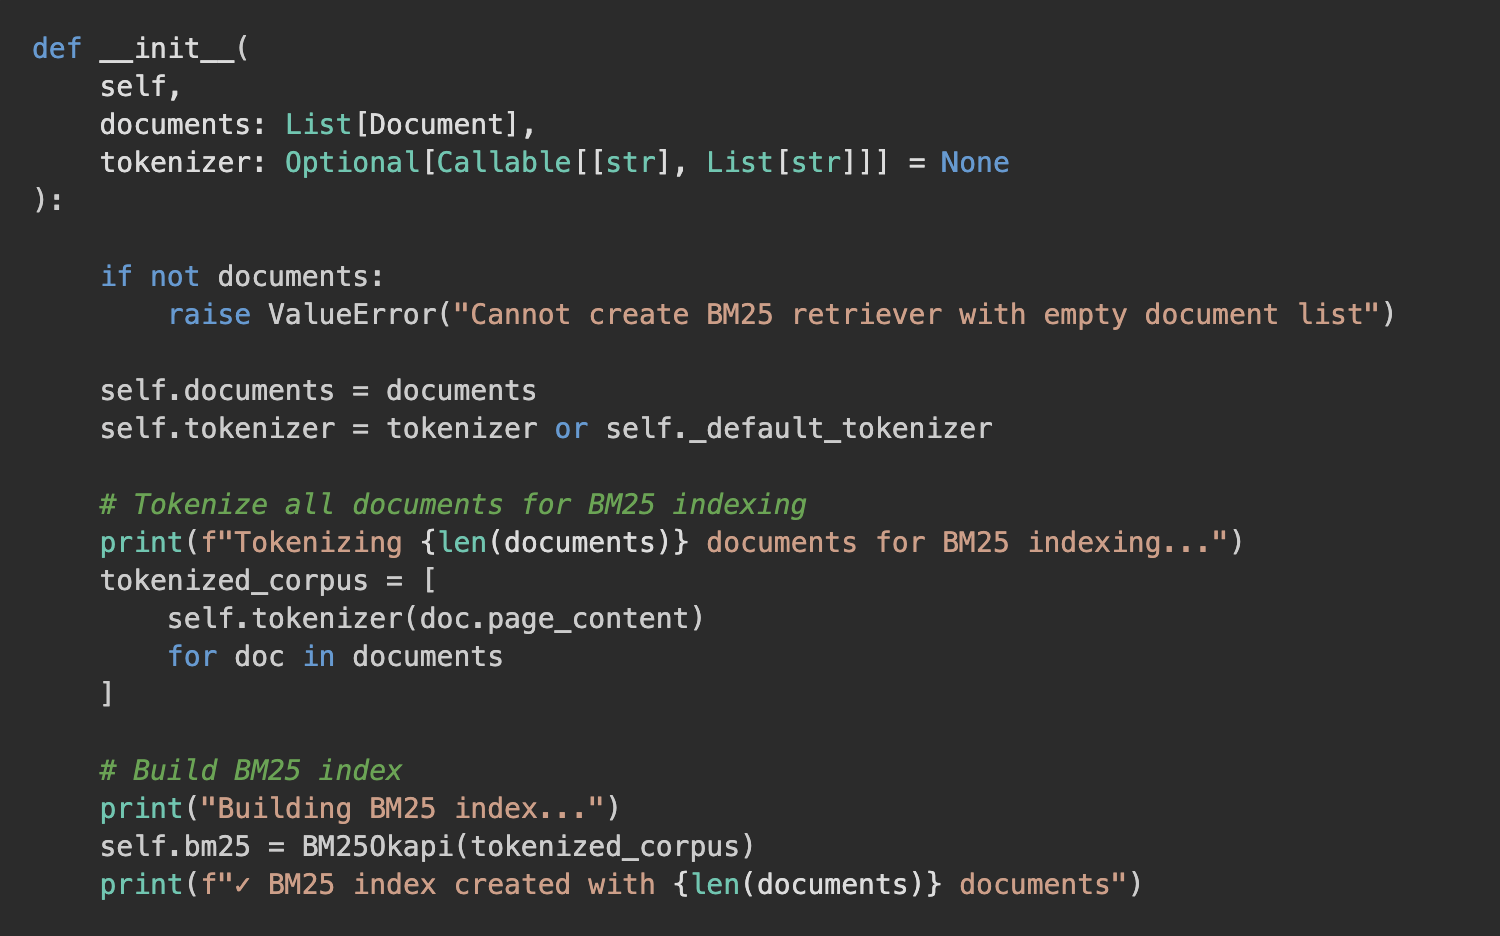
\includegraphics[width=1.0\textwidth]{figures/bm25_index_initialization_with_corpus_tokenization.png}
  \caption{BM25 index initialization with corpus tokenization}
  \label{fig:fig28b}
\end{figure}

\begin{figure}[H]
  \centering
  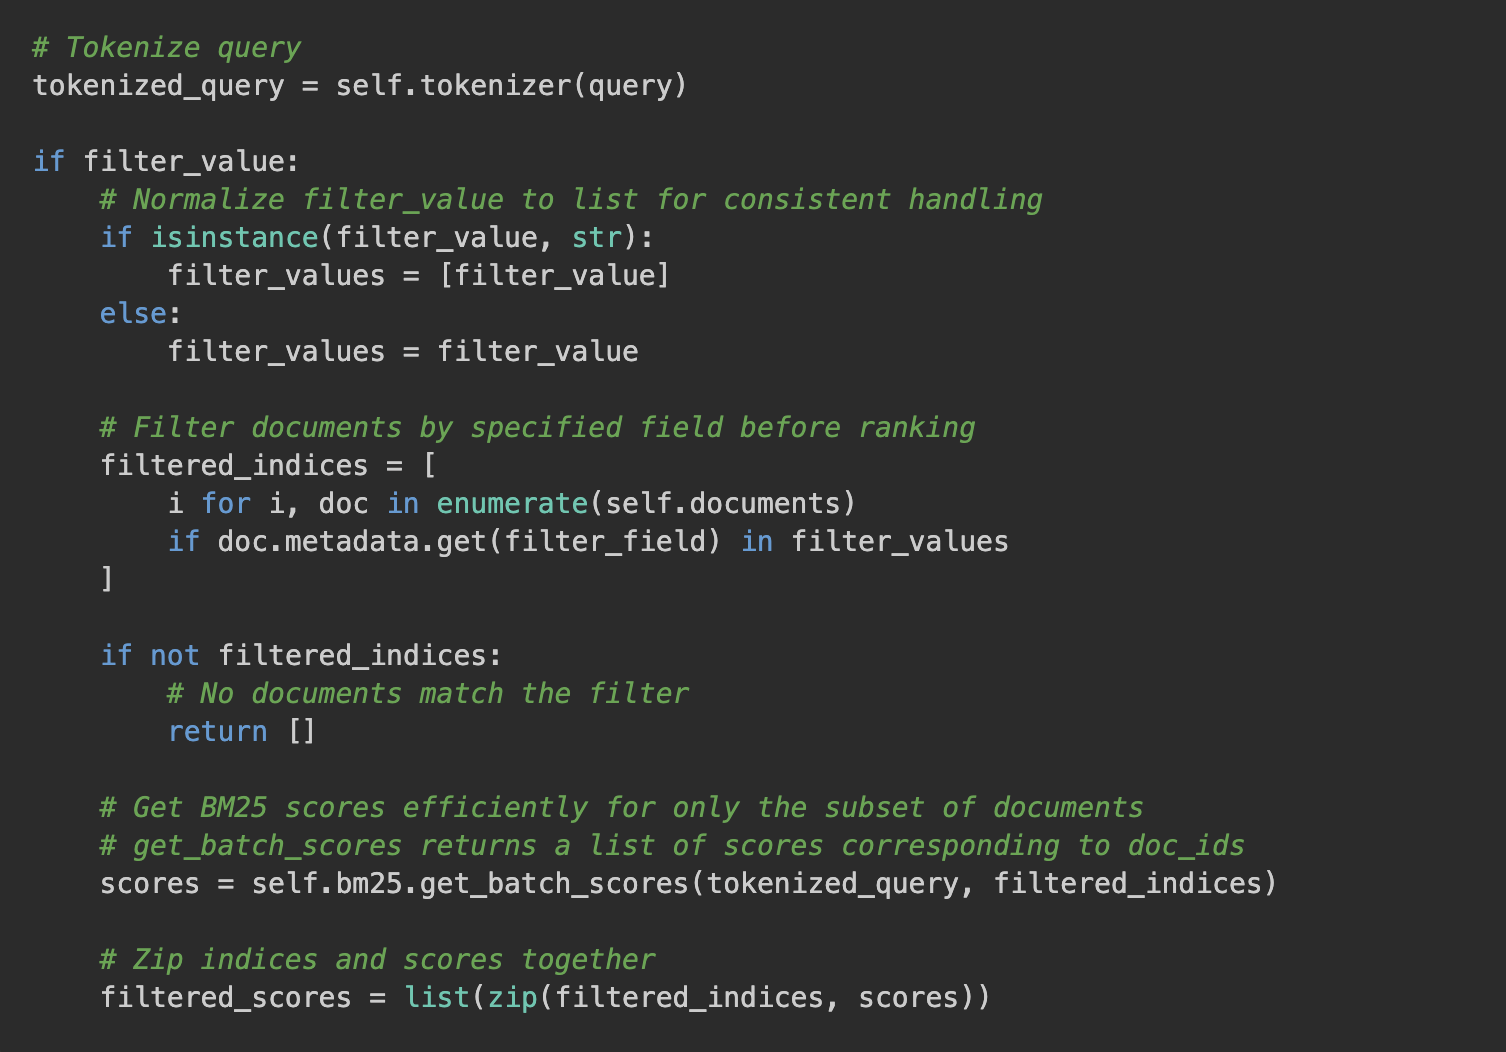
\includegraphics[width=1.0\textwidth]{figures/bm25_query_tokenization_and_metadata_filtering.png}
  \caption{BM25 query tokenization and metadata filtering}
  \label{fig:fig28c}
\end{figure}

Phonetic search uses Double Metaphone to recover recall when ASR output preserves pronunciation but not spelling, especially for names and rare technical vocabulary.\cite{black2021doublemetaphone,metaphone_pypi}

\begin{figure}[H]
  \centering
  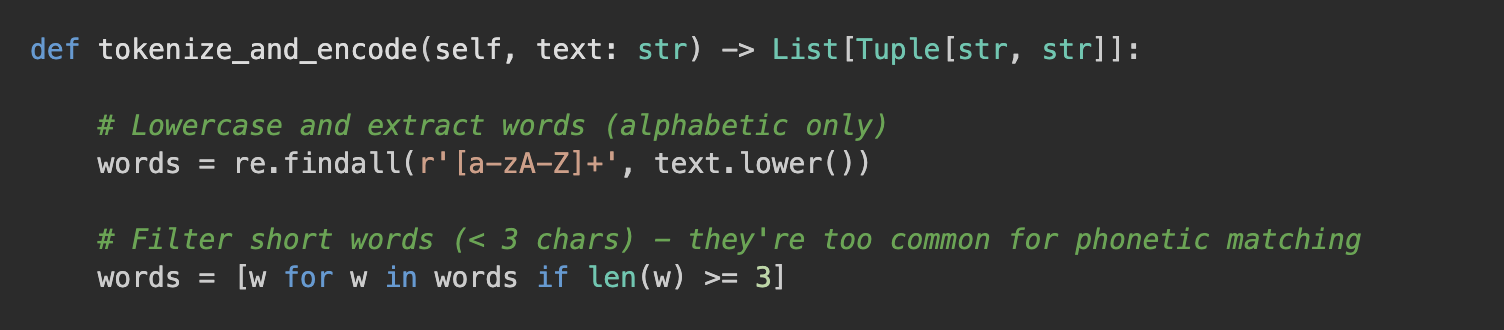
\includegraphics[width=1.0\textwidth]{figures/phonetic_word_tokenization_and_filtering.png}
  \caption{Phonetic word tokenization and filtering}
  \label{fig:fig29b}
\end{figure}

\begin{figure}[H]
  \centering
  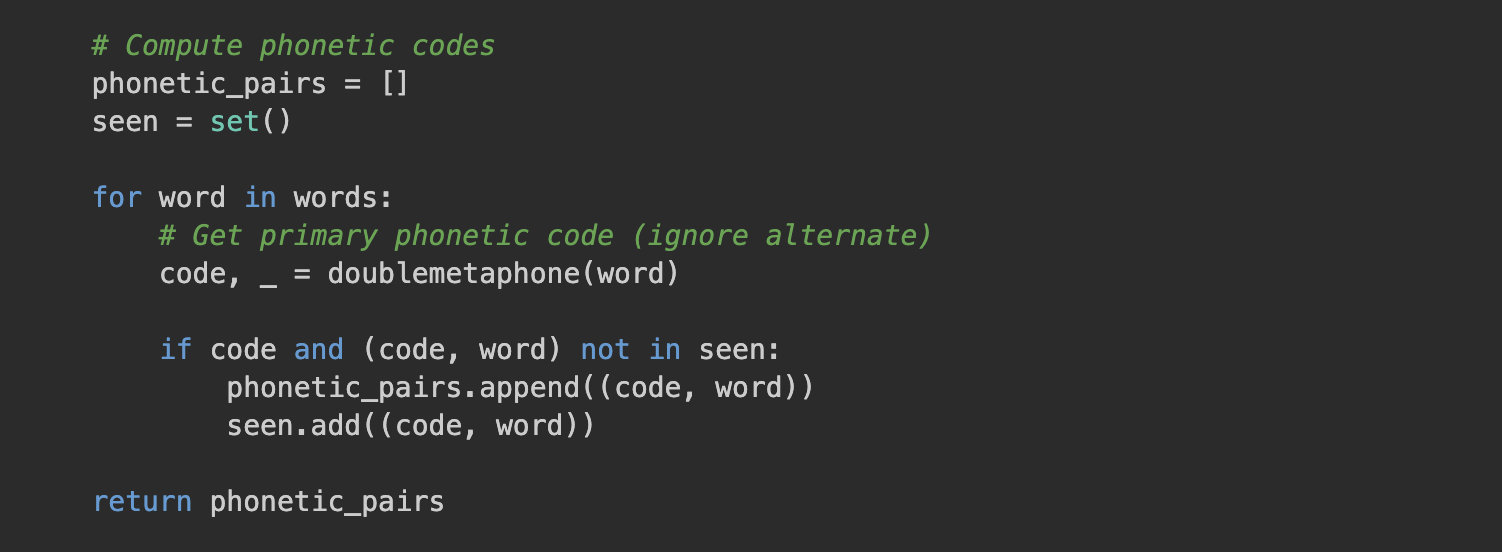
\includegraphics[width=1.0\textwidth]{figures/double_metaphone_phonetic_encoding.png}
  \caption{Double Metaphone phonetic encoding}
  \label{fig:fig29c}
\end{figure}

\begin{figure}[H]
  \centering
  
\includegraphics[width=1.0\textwidth]{figures/phonetic_encoding_examples_for_homophone_matching.png}
  \caption{Phonetic encoding examples for homophone matching}
  \label{fig:fig31}
\end{figure}

\begin{figure}[H]
  \centering
  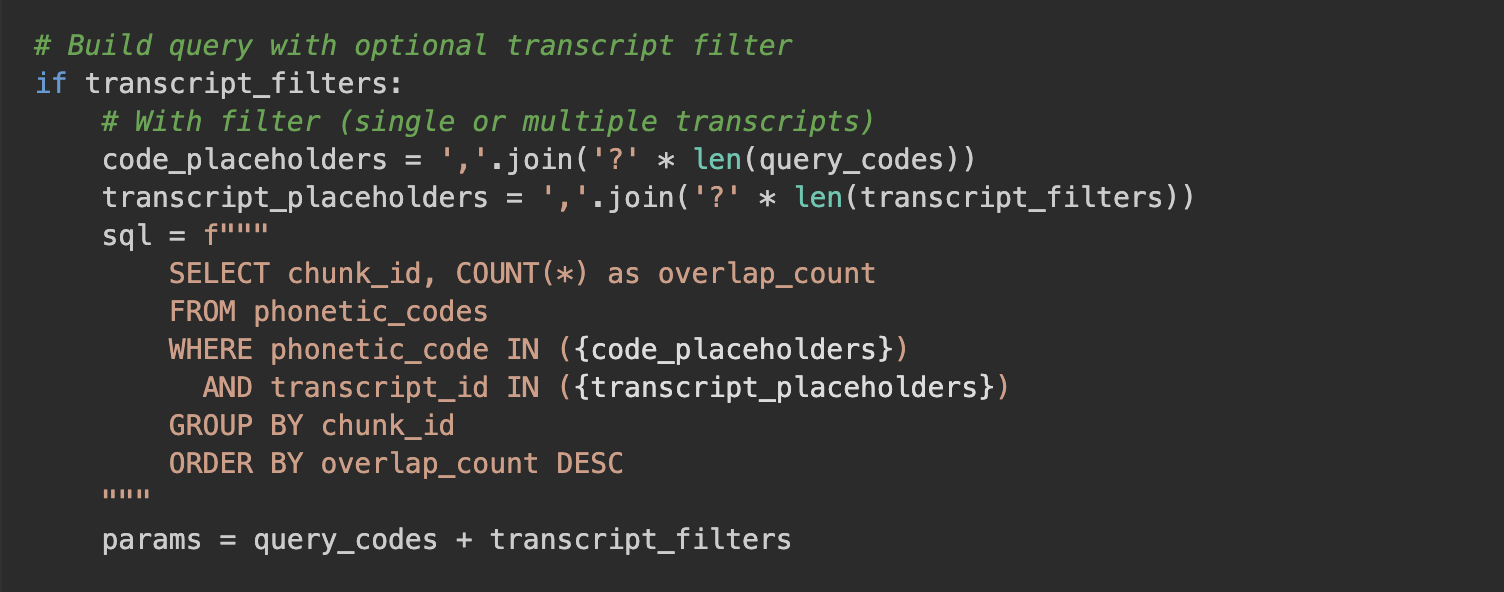
\includegraphics[width=1.0\textwidth]{figures/phonetic_retrieval_sql_query_with_transcript_filtering.png}
  \caption{Phonetic retrieval SQL query with transcript filtering}
  \label{fig:fig29e}
\end{figure}

\begin{figure}[H]
  \centering
  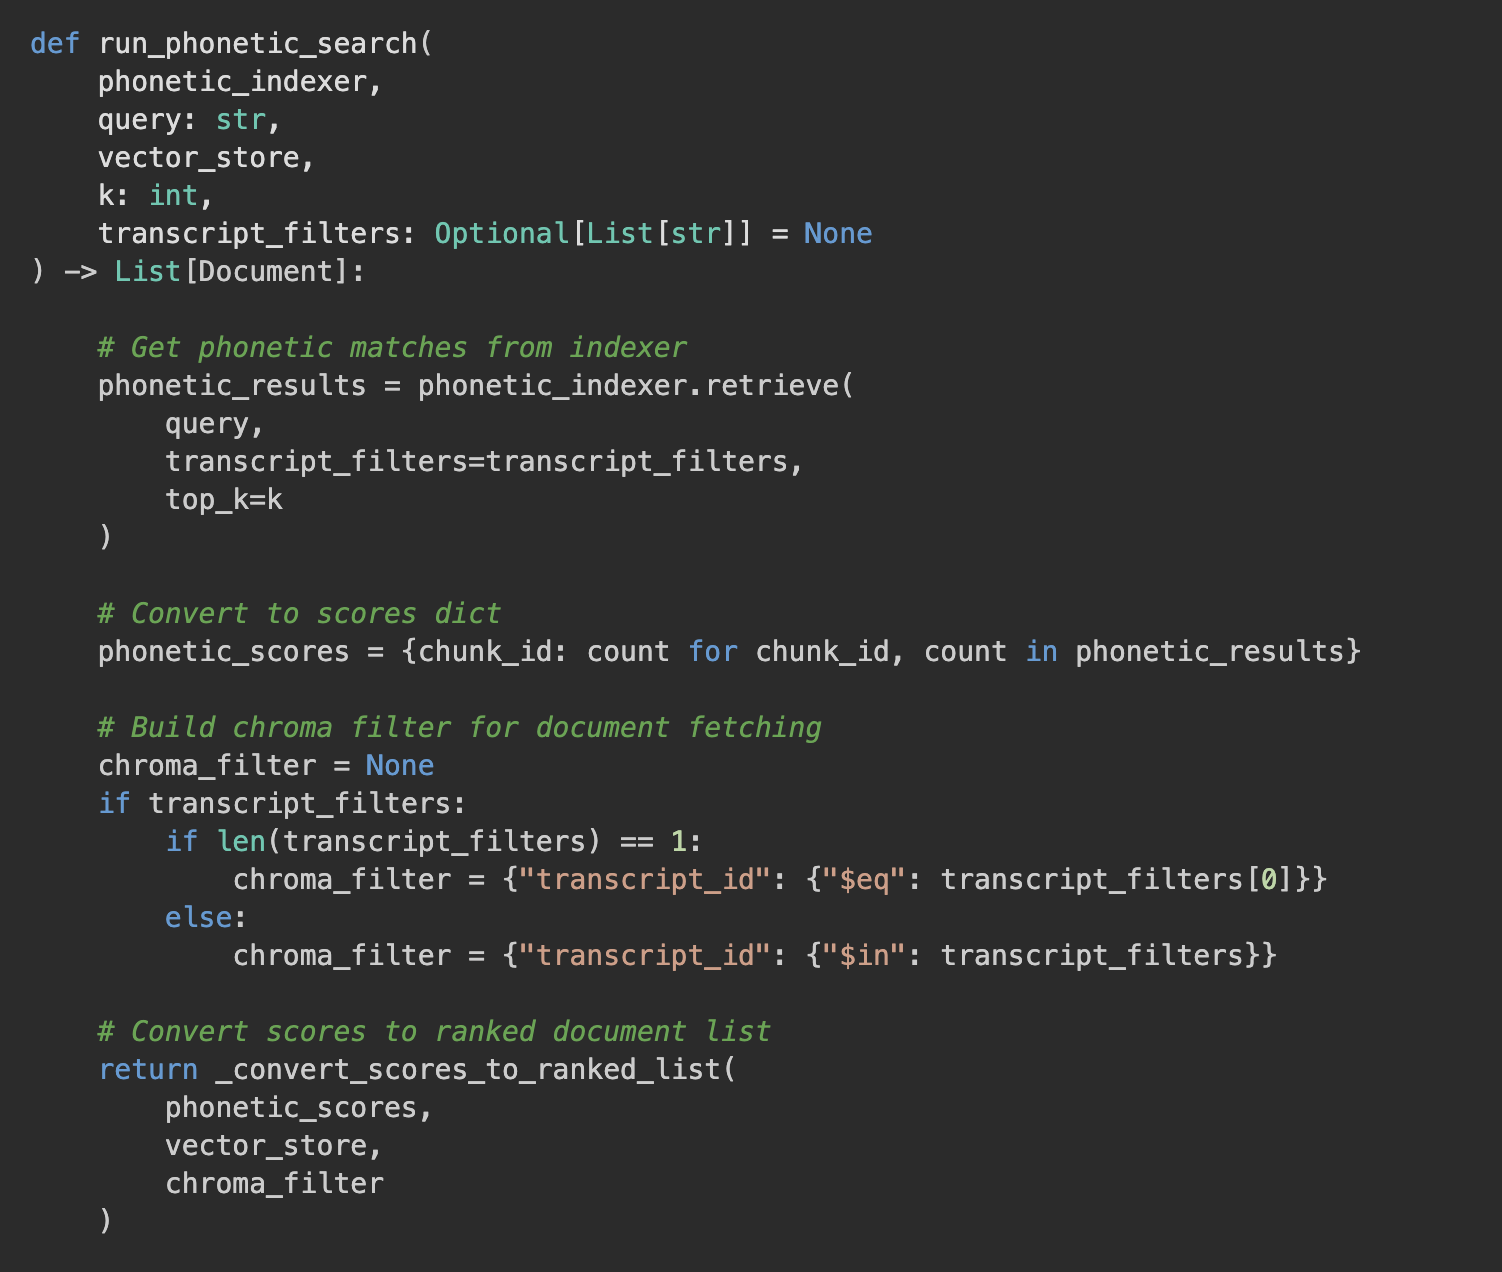
\includegraphics[width=1.0\textwidth]{figures/phonetic_score_conversion_and_document_retrieval.png}
  \caption{Phonetic score conversion and document retrieval}
  \label{fig:fig29g}
\end{figure}

Fuzzy matching complements phonetic search by using edit-distance similarity over rare tokens detected with Zipf frequency. This keeps the computation targeted toward tokens most likely to contain ASR errors or spelling variation.\cite{rapidfuzz_docs,wordfreq_pypi}

\begin{figure}[H]
  \centering
  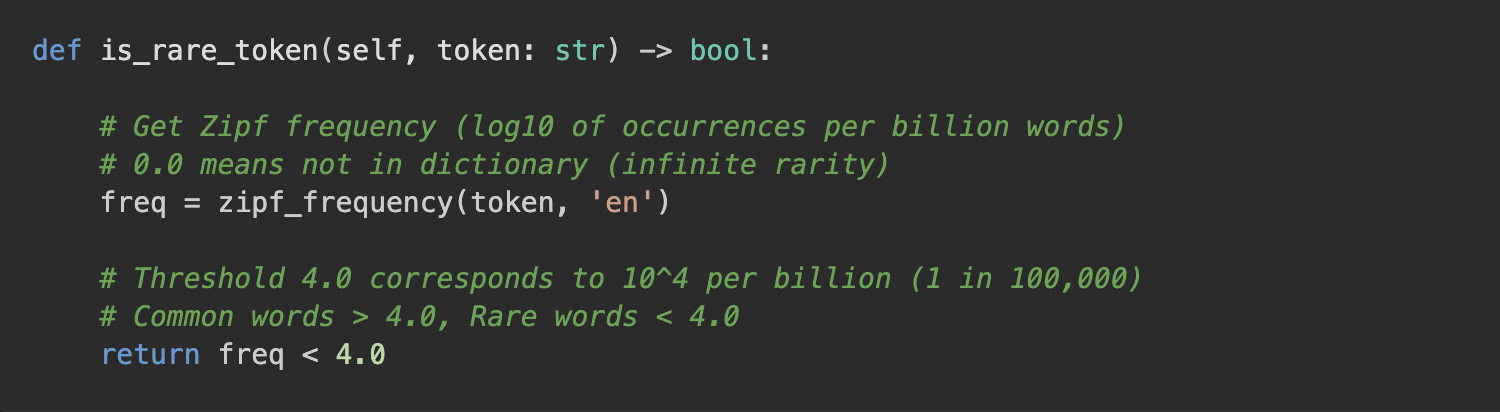
\includegraphics[width=1.0\textwidth]{figures/rare_token_detection_using_zipf_frequency.png}
  \caption{Rare token detection using Zipf frequency}
  \label{fig:fig30a}
\end{figure}

\begin{figure}[H]
  \centering
  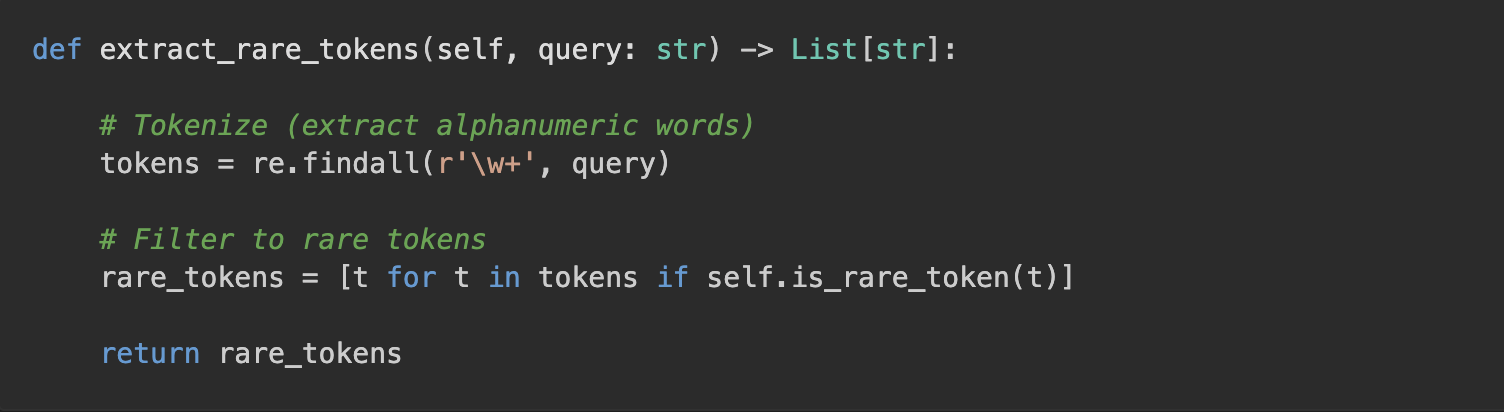
\includegraphics[width=1.0\textwidth]{figures/extracting_rare_tokens_from_query.png}
  \caption{Extracting rare tokens from query}
  \label{fig:fig30b}
\end{figure}

\begin{figure}[H]
  \centering
  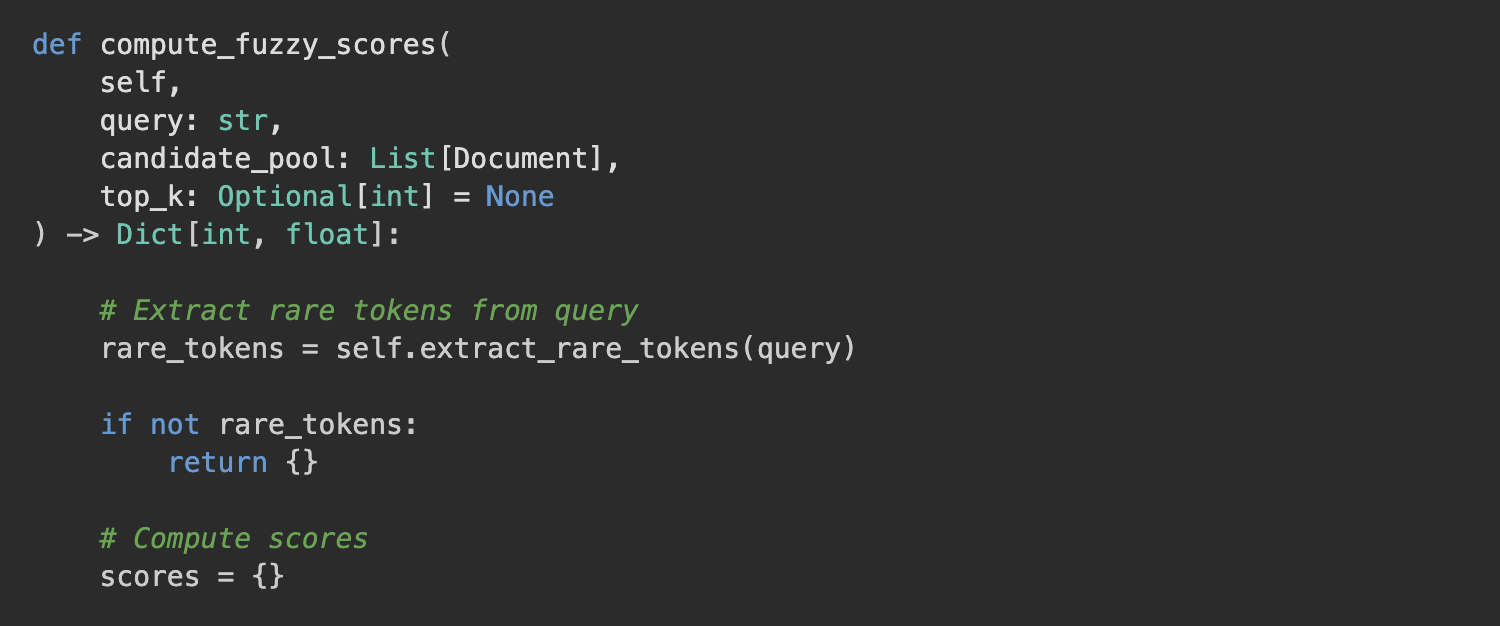
\includegraphics[width=1.0\textwidth]{figures/fuzzy_scoring_algorithm_setup_and_initialization.png}
  \caption{Fuzzy scoring algorithm: setup and initialization}
  \label{fig:fig30d}
\end{figure}

\begin{figure}[H]
  \centering
  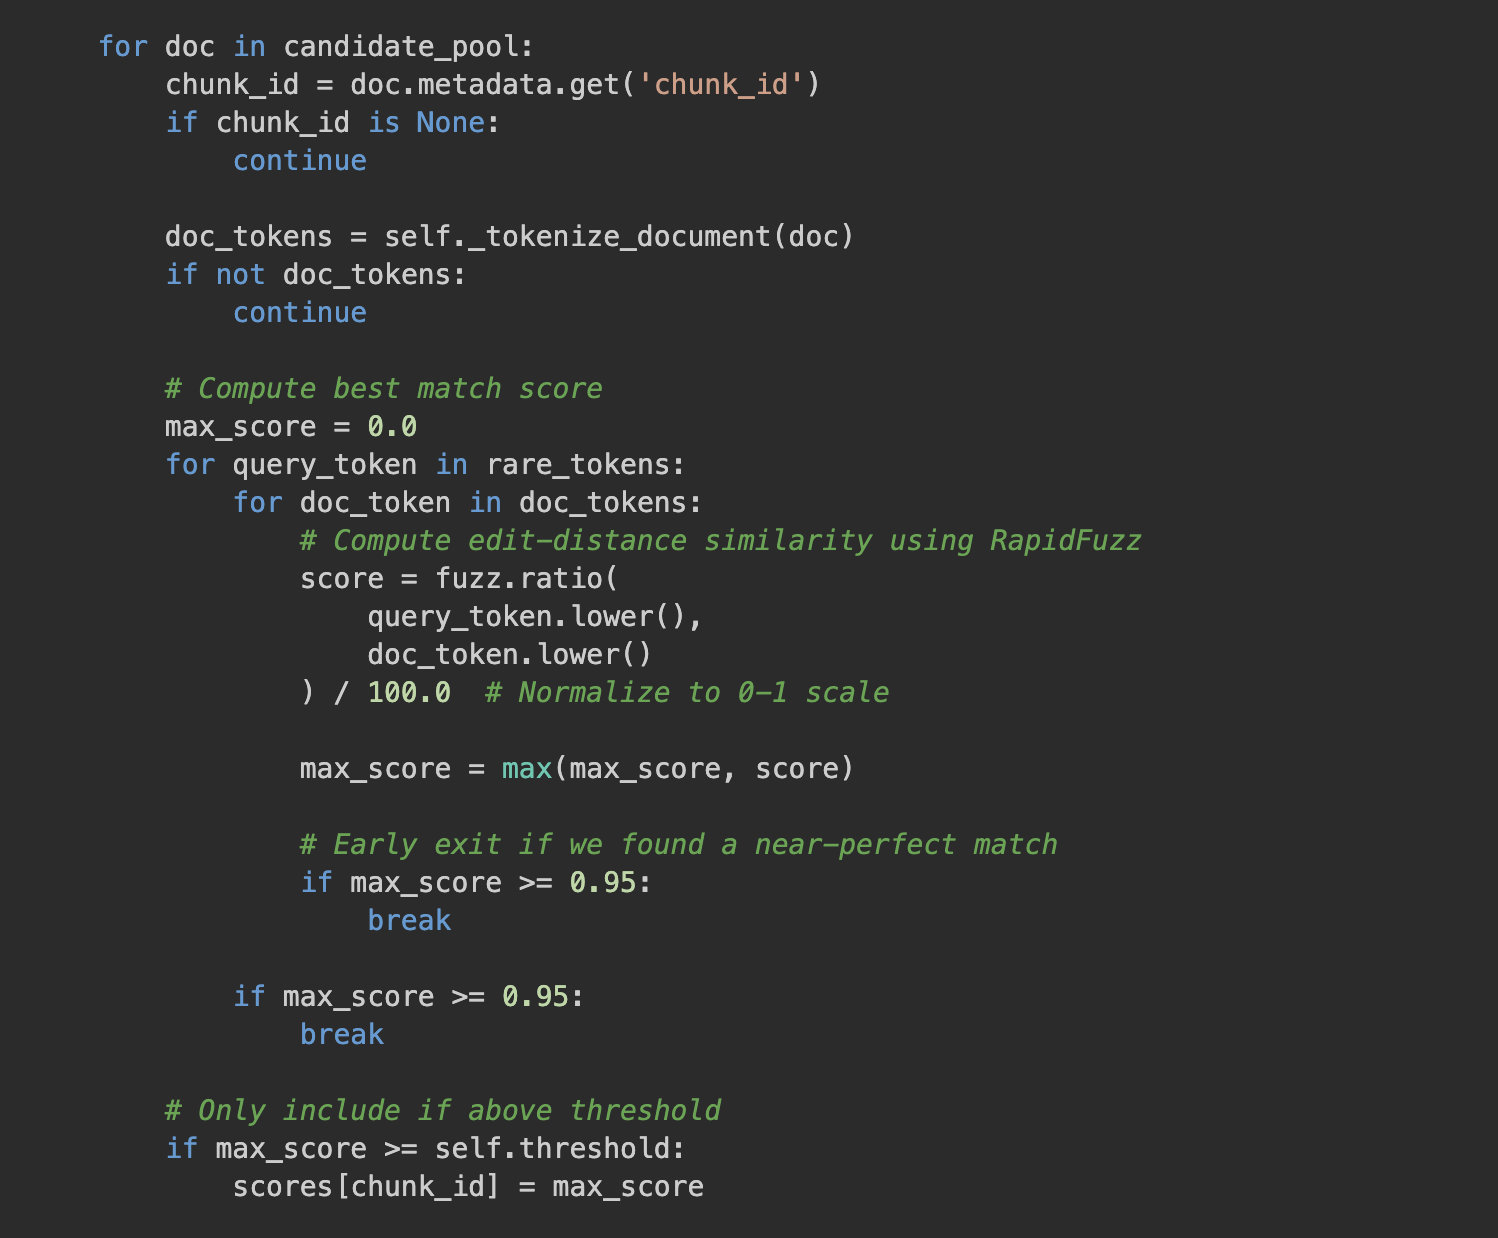
\includegraphics[width=1.0\textwidth]{figures/fuzzy_scoring_algorithm_nested_loop_with_rapidfuzz_ratio.png}
  \caption{Fuzzy scoring algorithm: nested loop with RapidFuzz ratio}
  \label{fig:fig30e}
\end{figure}

\begin{figure}[H]
  \centering
  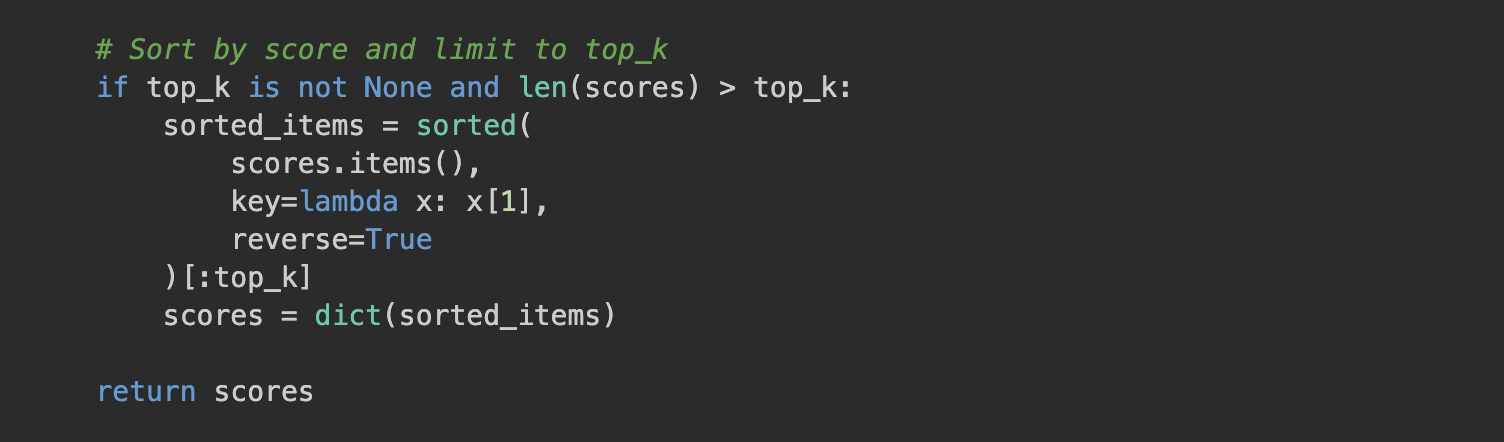
\includegraphics[width=1.0\textwidth]{figures/fuzzy_top_k_selection_and_ranking.png}
  \caption{Fuzzy top-k selection and ranking}
  \label{fig:fig30f}
\end{figure}

These four retrievers operate independently and are therefore executed in parallel before their results are fused. Table \ref{tab:search-method-characteristics} summarizes their respective roles, index types, and scoring signals.

\begin{table}[H]
  \centering
  \setlength{\tabcolsep}{4pt}
  \renewcommand{\arraystretch}{1.15}
  \begin{tabular}{|
    >{\centering\arraybackslash}m{0.16\textwidth}|
    >{\centering\arraybackslash}m{0.19\textwidth}|
    >{\centering\arraybackslash}m{0.16\textwidth}|
    >{\centering\arraybackslash}m{0.14\textwidth}|
    >{\centering\arraybackslash}m{0.07\textwidth}|
    >{\centering\arraybackslash}m{0.20\textwidth}|
  }
    \hline
    \textbf{Search Method} & \textbf{Algorithm} & \textbf{Index Type} & \textbf{Scoring Metric} & \textbf{Top-K} & \textbf{Best For} \\
    \hline
    Vector Search & Cosine similarity over embeddings & Dense vectors (Chroma) & Embedding distance & 10 & Semantic similarity, paraphrasing \\
    \hline
    BM25 Search & Probabilistic TF-IDF ranking & Inverted index & BM25 score & 25 & Keyword matching, proper nouns \\
    \hline
    Phonetic Search & Double Metaphone encoding & SQLite phonetic index & Overlap count & 10 & ASR errors, homophones \\
    \hline
    Fuzzy Matching & Edit-distance (RapidFuzz) & No index (full scan) & Fuzzy ratio & 10 & Typos, spelling variations \\
    \hline
  \end{tabular}
  \caption{Search method characteristics in the hybrid retrieval stage used by the RAG subsystem}
  \label{tab:search-method-characteristics}
\end{table}

After Stage 1 retrieval, the system applies Reciprocal Rank Fusion to normalize heterogeneous rankings and reward candidates that score well across multiple retrieval signals.\cite{cormack2009reciprocal}

\begin{figure}[H]
  \centering
  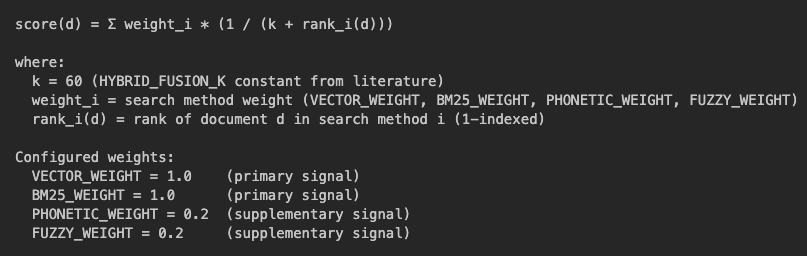
\includegraphics[width=1.0\textwidth]{figures/reciprocal_rank_fusion_weights_for_hybrid_retrieval_signals.png}
  \caption{Reciprocal Rank Fusion weights for the hybrid retrieval signals}
  \label{fig:fig35}
\end{figure}

The fused pool is then reranked with a cross-encoder, which jointly scores each query-document pair and provides a more precise final ordering than the initial retrieval signals alone.\cite{nogueira2019passage}

\begin{figure}[H]
  \centering
  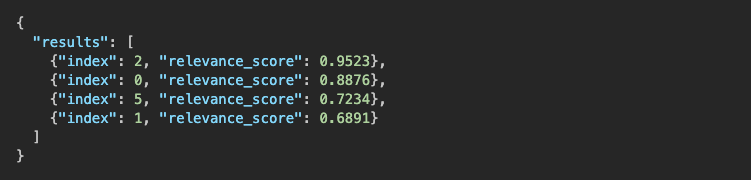
\includegraphics[width=1.0\textwidth]{figures/expected_response_format.png}
  \caption{Expected reranker response format}
  \label{fig:fig38a}
\end{figure}

\begin{figure}[H]
  \centering
  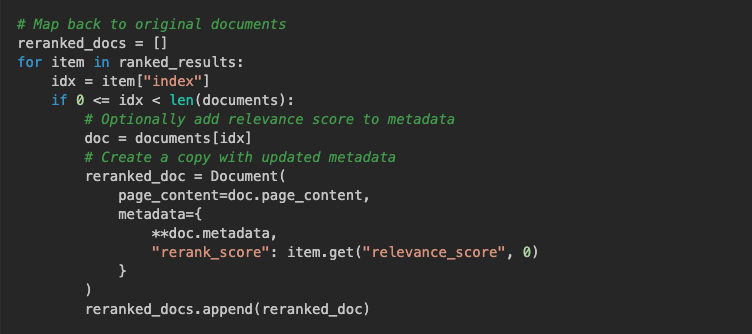
\includegraphics[width=1.0\textwidth]{figures/mapping_results_to_original_documents.png}
  \caption{Mapping reranked results back to the original documents}
  \label{fig:fig38c}
\end{figure}

\begin{figure}[H]
  \centering
  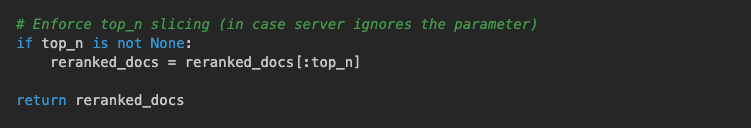
\includegraphics[width=1.0\textwidth]{figures/top_n_selection.png}
  \caption{Top-n selection after reranking}
  \label{fig:fig38d}
\end{figure}

\section{Context Formatting and Prompt Construction}
After reranking, the selected chunks are converted into a structured context string for answer generation. Each chunk is formatted with identifiers and timestamps so that the generated answer remains auditable against the source transcript.

\begin{figure}[H]
  \centering
  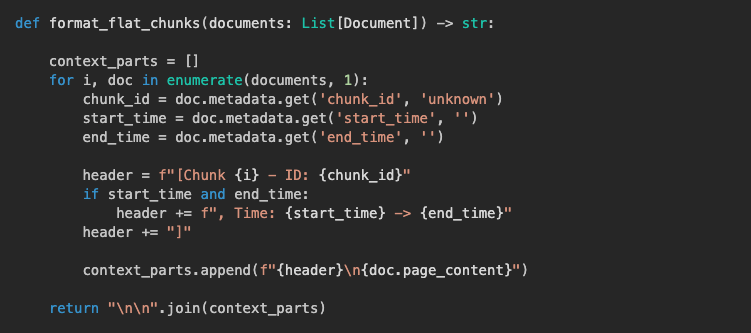
\includegraphics[width=1.0\textwidth]{figures/chunk_formatting_with_individual_metadata_headers.png}
  \caption{Chunk formatting with individual metadata headers}
  \label{fig:fig40a}
\end{figure}

\begin{figure}[H]
  \centering
  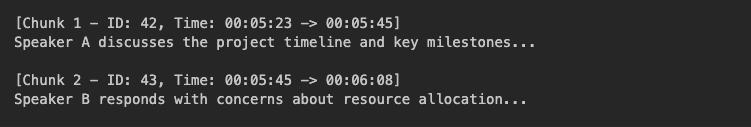
\includegraphics[width=1.0\textwidth]{figures/output_format_example.png}
  \caption{Output format example}
  \label{fig:fig40b}
\end{figure}

\begin{figure}[H]
  \centering
  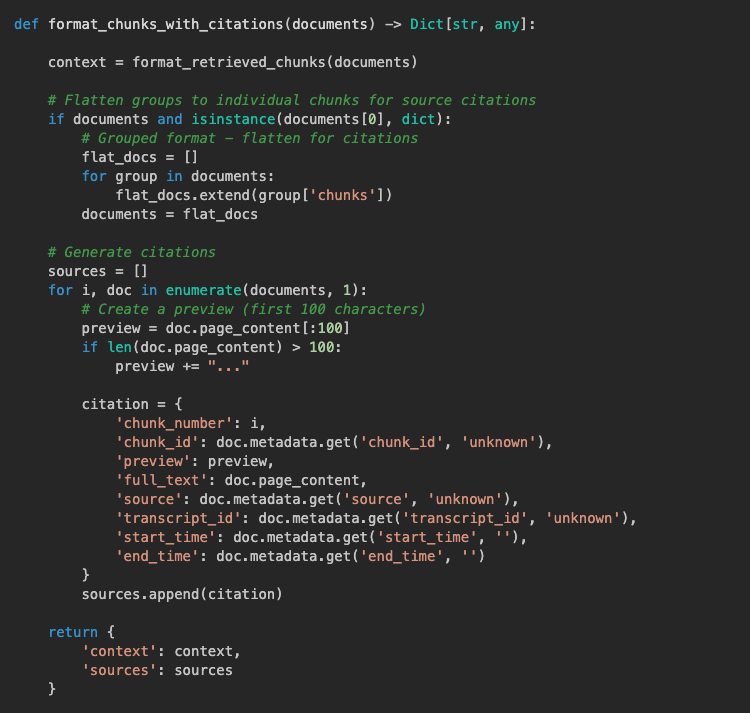
\includegraphics[width=1.0\textwidth]{figures/citation_formatting_for_user_transparency_and_source_attribution.png}
  \caption{Citation formatting for user transparency and source attribution}
  \label{fig:fig40d}
\end{figure}

The prompt layer combines system instructions, retrieved context, optional chat history, and the current user question. For broad or ambiguous requests, the same prompt-construction path can also inject summary-derived transcript framing before answer generation.\cite{langchain_prompts,langchain_chatprompt,langchain_messages_placeholder}

\begin{figure}[H]
  \centering
  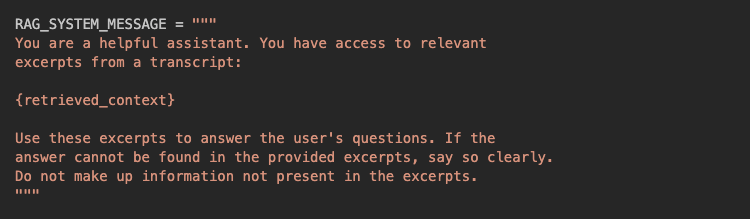
\includegraphics[width=1.0\textwidth]{figures/rag_system_message_template_defining_assistant_role_and_constraints.png}
  \caption{Grounded QA system message template defining assistant role and constraints}
  \label{fig:fig42a}
\end{figure}

\begin{figure}[H]
  \centering
  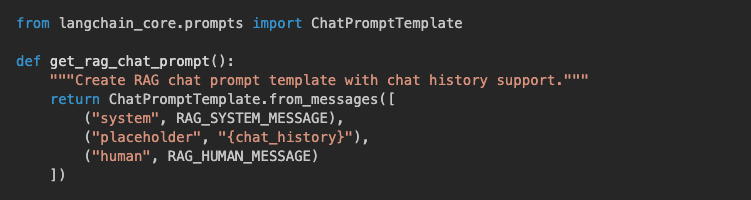
\includegraphics[width=1.0\textwidth]{figures/complete_rag_chat_prompt_construction_with_history_support.png}
  \caption{Complete RAG chat prompt construction with history support}
  \label{fig:fig42c}
\end{figure}

\begin{figure}[H]
  \centering
  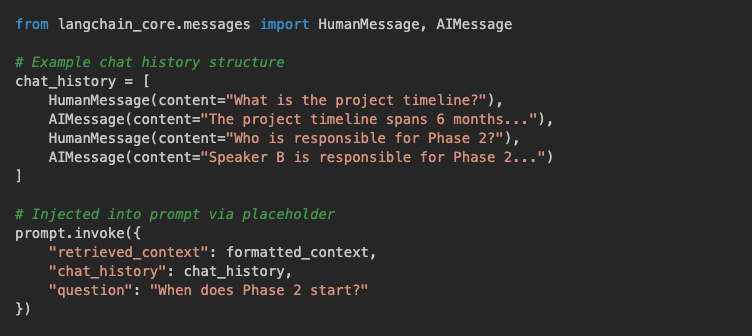
\includegraphics[width=1.0\textwidth]{figures/chat_history_structure_for_multi_turn_conversation_support.png}
  \caption{Chat history structure for multi-turn conversation support}
  \label{fig:fig42d}
\end{figure}

\begin{figure}[H]
  \centering
  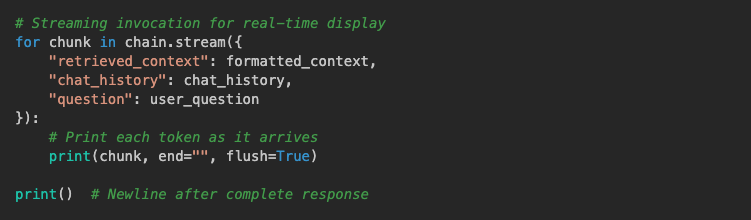
\includegraphics[width=1.0\textwidth]{figures/streaming_response_handling_for_real_time_token_display.png}
  \caption{Streaming response handling for real-time token display}
  \label{fig:fig43d}
\end{figure}
